\chapter{Egyensúlyozás}\label{ch:EGYENSULY}
\begin{osszefoglal}
E fejezet célja, hogy bemutassa a PID szabályzó algoritmus működését. E mellet sorkelűr az egyensúlyozás működésének leírására, valamint hogy miként lehet felhasználni ez esetbe a PID szabályzó algoritmust.
\end{osszefoglal}

\section{PID szabályzó algoritmus}\label{sec:EGYENSULY:pid}

A szabályzó rendszereket kétféleképpen nevezhetjük nyílt vagy zárt ciklusosnak.  Nyílt ciklusos rendszerek esetén nincs visszacsatolás, ezért nem megfelelő komplex problémák megoldására. Előnyös a használata kisebb kapacitás esetén, mivel alacsony költségű. A zárt ciklusos rendszerek visszacsatolással működnek, vagyis a rendszer kimenetének hatására visszajelzést kapunk.

A PID\texttt{(Proportional Integral Derivate)} elterjedt zárt ciklusos rendszer, az ipari szabályzó körökben köszönhetően a viszonylag egyszerű félépítésének és a könnyen kezelhetőségének. Számos felhasználási lehetősége van, ilyenek a nyomás, hőmérséklet, sebesség szabályozás. E szabályzó rendszer bementi értéke az aktuális hiba.

A hibát az elvárt érték és az aktuális érték különbsége határoz meg. Esetünkben az aktuális értékek a következők: robot dőlési szöge, szög változásának sebessége, a robot pozíciója illetve sebessége. Az előbb felsorolt értékek esetén az elvárt értékek ahhoz, hogy a robot egyensúlyi állapotba maradjon 0-hoz kell közelítsenek.

A szabályzó kimeneti értéke a motorokra leadott erő. Esetünkbe tehát a visszacsatolás az előbb felsorolt négy értékben nyilvánul meg, mivel a kerekre leadott erő befolyásolja ezen értékeket.

A PID, mint a nevéből is látható három tagból tevődik össze: P \texttt{(Proportional)} az arányos tag, I \texttt{(Integral)} a hibák integrált tagja és a D \texttt{(Derivate)} a hibák időbeli változásának derivált tagja. Abban az esetben ha az előbb felsorolt tagok közül nem vesszünk figyelembe minden tagot, akkor a következő szabályzókról beszélhetünk: P, PI és PD.

PID szabályzó matematikai képlete: $$u(t)=K_{P}e(t)+K_{I}\int e(t)dt+K_{D}\frac{d}{dt}e(t),$$ ahol $t$ jelöli az időt, $e(t)$ a bemeneti hibát illetve az $u(t)$ a kimenet. A $K_{P}, K_{I}, K_{D}$ paraméterek rendre az arányos, integrált és a derivált tagok súlya, amelyek meghatározásakor a szabályzó érzékenységét valamint befolyásolják teljesítményét.

Kizárólag az arányos tag használata esetén a szabályzó rendszer olyan eseteknél használható, ahol megengedett egy bizonyos nagyságú hiba az kimenetben miután a rendszer stabilizálódott. Az arányos tag paramétere a $K_{P}$, amely egy konstans érték, ha túl nagy instabil rendszert eredményez.

Az integrált tag önmagában nem használható mint az arányos tag. Az integrált tag esetén a hibák összege mind addig változik míg az arányos tag nulla nem lesz. Tehát a feladata, hogy egy pontosabb és precízebb szabályzó rendszer biztosítása. Mivel kód szinten nem valósítható meg az integrálás ezért a következő képlet segítségével közelítsük meg:$$u(t)=K_{I}\cdot\sum e(t),$$ ahol az előbbihez hasonlóan $K_{I}$ konstans.

A derivált tag értéke arányos a hiba változási sebességével. Feladata a hirtelen változások késleltetése, ezáltal egy stabilabb rendszert biztosítva. Ez esetben is felmerül az előbb említett probléma ugyan is kód szinten a deriválás sem valósítható meg ezért a következő képlettel közelítsük meg:$$u(t)=K_{D}\cdot (e(t) - e(t-1),$$ ahol szintén a $K_{D}$ konstans.

A \ref{pidFig} ábrán látható a PID szabályzó tagjainak változása egy teszt esetén. Jól látható az ábrán, hogy a derivált tag ellentétes előjelű az arányos taghoz viszonyítva, ennek köszönhetően a hirtelen változások késleltetve lesznek. Az integrált tag és az arányos tag esetén jól látható, hogy a hasonló oszcillációt végeznek.

\begin{figure}[!hp]
	\centering
	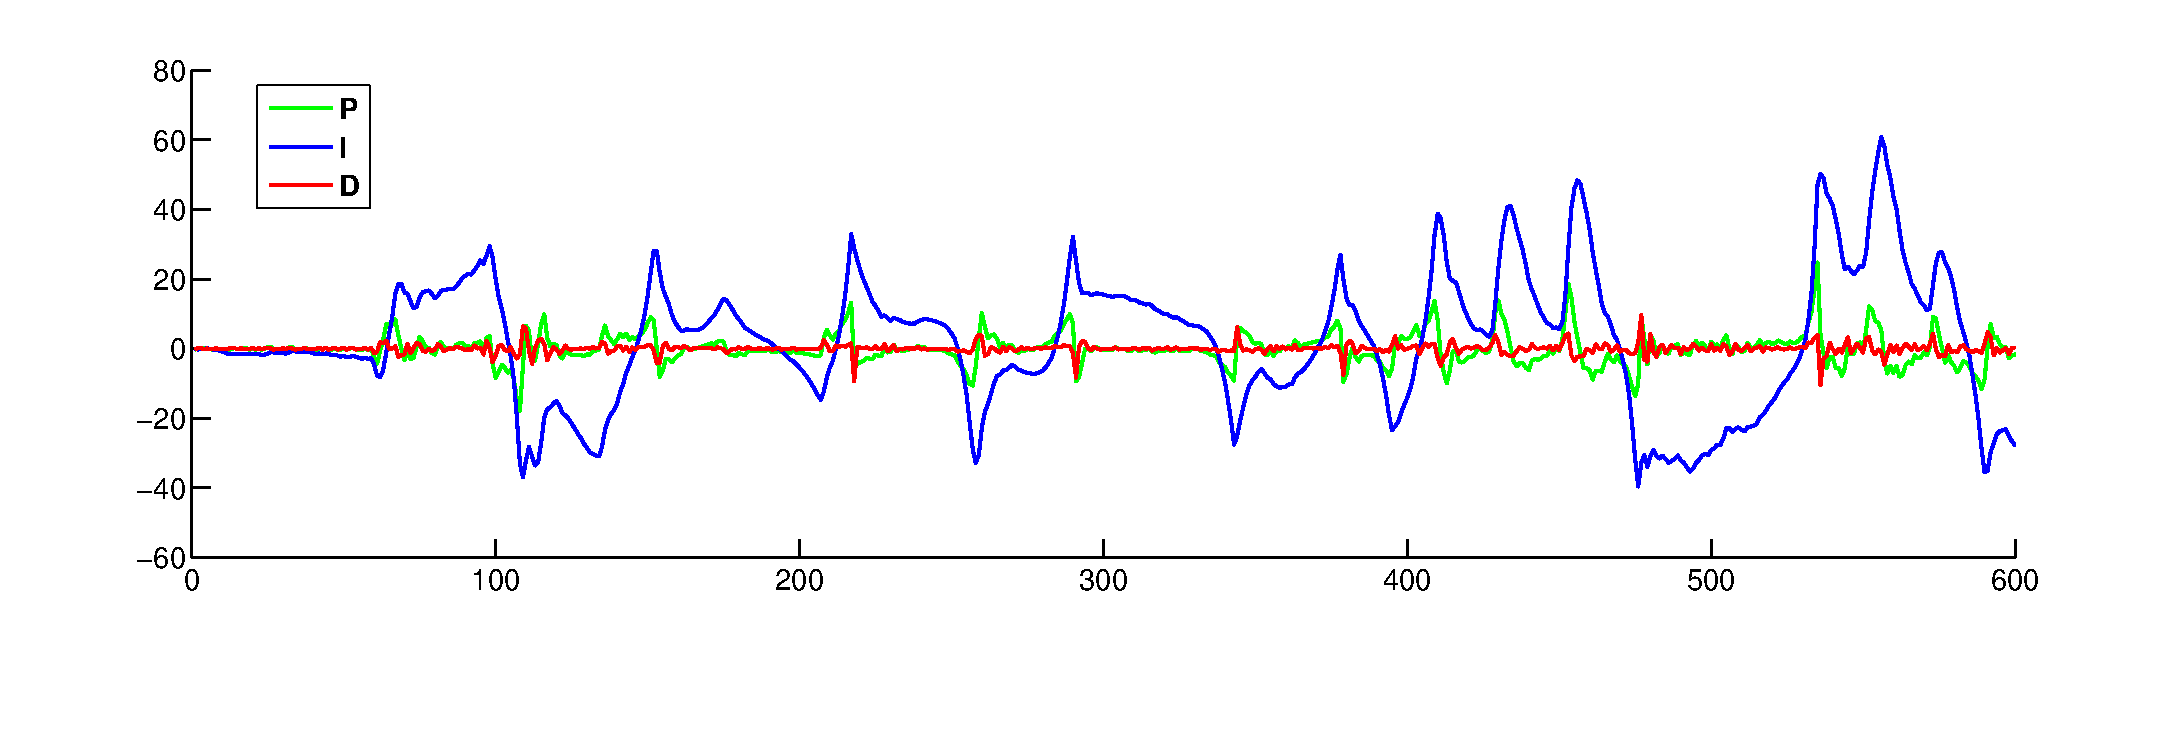
\includegraphics[width=1\linewidth]{images/pid.eps}
	\captionsetup{justification=centering,margin=1.5cm}
	\caption[Egy tesz során kapott PID tagjainak értékeit ábrázolja]
	{Egy tesz során kapott PID tagjainak értékeit ábrázolja. Az x tengelyen jelöljük a iterációk számát,	az y tengelyen a PID tagok értékének mértékét.}
	\label{pidFig}
\end{figure}
